\documentclass{article}

\usepackage{arxiv}

\usepackage[utf8]{inputenc} % allow utf-8 input
\usepackage[T1]{fontenc}    % use 8-bit T1 fonts
\usepackage{hyperref}       % hyperlinks
\usepackage{url}            % simple URL typesetting
\usepackage{booktabs}       % professional-quality tables
\usepackage{amsfonts}       % blackboard math symbols
\usepackage{nicefrac}       % compact symbols for 1/2, etc.
\usepackage{microtype}      % microtypography

\usepackage{graphicx}
\usepackage{amsmath}

\newtheorem{definition}{Definition}
\newtheorem{lemma}{Lemma}
\newtheorem{proposition}{Proposition}
\newtheorem{program}{Program}
\newtheorem{convention}{Convention}

\title{Notes on geometrical interpretation of adjoint equation}

%\date{September 9, 1985}	% Here you can change the date presented in the paper title
%\date{} 					% Or removing it

\author{
  Mingli~Yuan \\
  AI Lab \\
  Beijing ColorfulClouds Tech.\\
  Beijing, 100083 \\
  \texttt{mingli.yuan@caiyunapp.com} \\
  %% examples of more authors
  %% \AND
  %% Coauthor \\
  %% Affiliation \\
  %% Address \\
  %% \texttt{email} \\
  %% \And
  %% Coauthor \\
  %% Affiliation \\
  %% Address \\
  %% \texttt{email} \\
  %% \And
  %% Coauthor \\
  %% Affiliation \\
  %% Address \\
  %% \texttt{email} \\
}

% Uncomment to remove the date
%\date{}

% Uncomment to override  the `A preprint' in the header
%\renewcommand{\headeright}{Technical Report}
%\renewcommand{\undertitle}{Technical Report}

\begin{document}
\maketitle

\begin{abstract}
Traditionally, adjoint equation was introduced via the technic of integration-by-parts.
After recalling the geometrical interpretation of adjoint operators in linear cases,
we reveal that adjoint equation shares the same interpretation,
and then a new dual-number-based definition of adjoint equation and proof for equivalence between definitions are given.
\end{abstract}

\keywords{adjoint \and adjoint equation \and geometrical interpretation \and dual number}

\section{Introduction}

The concept of adjoint is very fundamental\cite{Daz1953MethodsOM}\cite{Marchuk1995}, and adjoint equation shows its importance in domains of optimal control\cite{Liberzon2012CalculusOV}, sensitivity analysis\cite{hall1983physical}, and data assimilation\cite{Errico1997WhatIA}. Also, recent contribution\cite{Chen2018NeuralOD} shows adjoint equation can play a role in the intersection area of deep learning and differential equations.

In linear cases, there is an apparent geometrical interpretation of adjoint operators, and in this paper, we want to reveal adjoint equation shares the same interpretation.

\subsection{Definition and geometrical interpretation of adjoint operators in linear case}

Formally, we can define a pair of adjoint operators in a dual system.

\begin{definition}
\label{d0}
A dual system $ \langle X, Y \rangle $ is a bilinear mapping $ \langle , \rangle : X \times Y \to F $ where $X$, $Y$ are two vector space and $ F $ is a field.
\end{definition}

Geometrically, We can interpret that $ X $ is a bottom space which holds the points, $ Y $ is a frame space which holds the coordinate frames, and the value of $ \langle x, y \rangle $ is the coordinate of $x$ under a frame $y$.

\begin{definition}
\label{d1}
For two dual system $ \langle X_1, Y_1 \rangle $ and $ \langle X_2, Y_2 \rangle $ , each of the two operator $ A : X_1 \to X_2$ and $ B : Y_2 \to Y_1 $ is an adjoint of the other counterpart,
if and only if, the equation
\begin{equation}
  \label{eq:langrangeidentity}
  \langle A \phi, \psi \rangle = \langle \phi, B \psi \rangle
\end{equation}
holds for arbitrary $ \phi \in X_1 $ and $ \psi \in Y_2 $
\end{definition}

Under the above interpretation, a pair of adjoint operators are just active and passive transformations (or alibi and alias transformations)\cite{wiki:aptrans}.

The left side of Equation \ref{eq:langrangeidentity} $ \langle A \phi, \psi \rangle $ is interpreted as an active transformation(operator) $ A $ act on a point $\phi$ in bottom space $ X_1 $ and hence have a coordinate $\langle A \phi, \psi \rangle$ after the transformations;

The right side of Equation \ref{eq:langrangeidentity} $ \langle \phi, B \psi \rangle $ is interpreted as a passive transformation(operator) $ B $ act on a frame $\psi$ in frame space $ Y_2 $ and hence have another coordinate $\langle \phi, B \psi \rangle$ after the transformations.

\begin{figure}[ht]
\label{fig:alias_and_alibi}
\centering
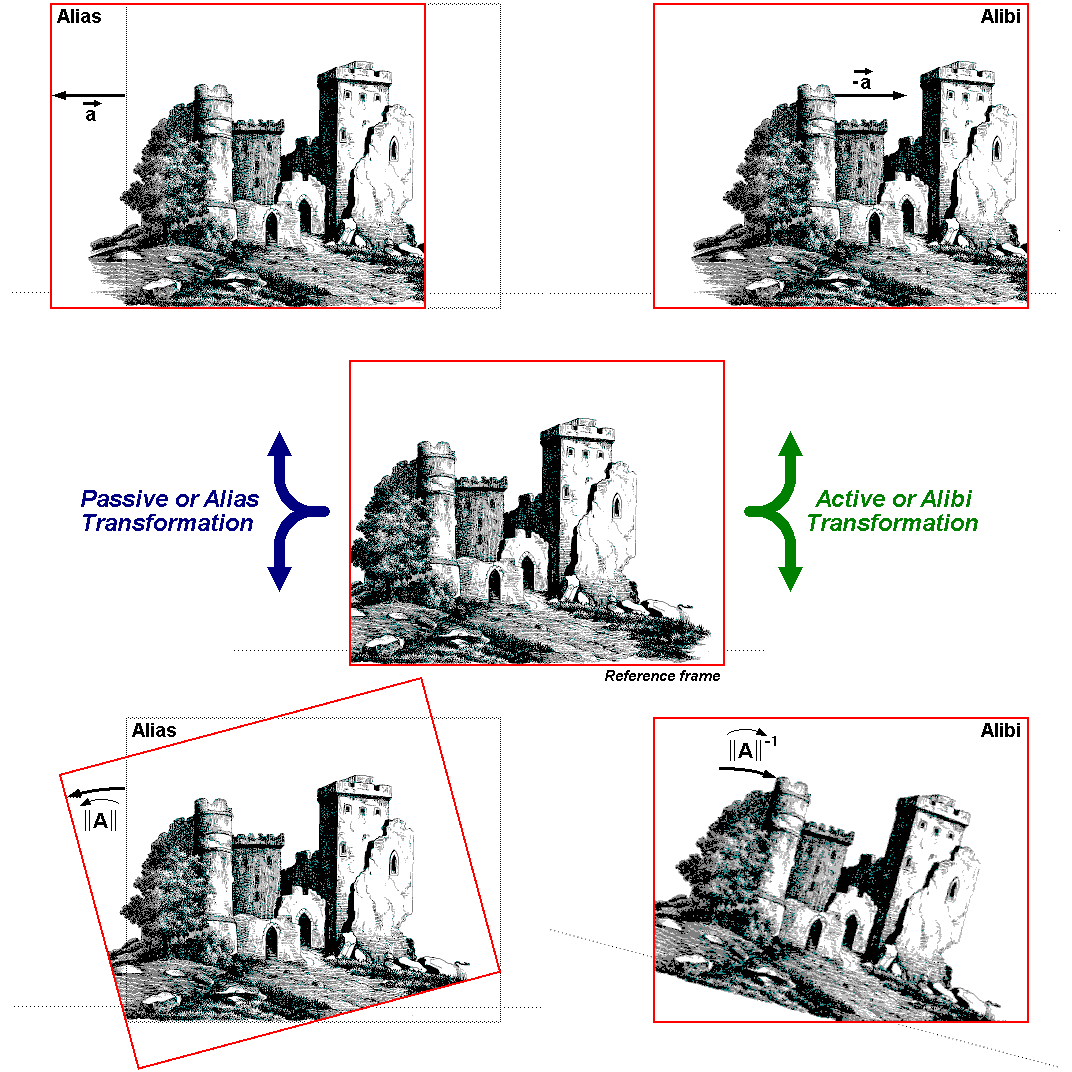
\includegraphics[width=3.5in]{../images/adjoint/alias_and_alibi.png}
\caption{A dual system and two pair of adjoint operators\cite{wiki:aatrans}}
\end{figure}

Then, the Equation \ref{eq:langrangeidentity} just says that the two coordinate are always the same, just as illustrated in Figure \ref{fig:alias_and_alibi}.

\subsection{Different problems leading to adjoint equation}

Adjoint equation is a tool when we seek an optimized solution bounded to an evolutionary differential equation.

\begin{equation}
\begin{array}{ll}
\dot{\mathbf{y}} = f(\mathbf{x}, t; \theta) & (\mathbf{x}, t) \in \Omega \times [0, 1] \\
\mathbf{y} = u(\mathbf{x}, t; \theta) & (\mathbf{x}, t) \in \partial \Omega \times [0, 1] \\
\end{array}
\end{equation}

The optimized solution can be a boundary value to apply control, or instead, an initial value to fit observations aftermath, or possibly, better parameters to influence the process.
In this section, we will show some typical problems appeared in different literatures ? \cite{Liberzon2012CalculusOV}\cite{hall1983physical}\cite{Errico1997WhatIA} ? and reformulate these problems with a uniformed notion.

\subsubsection{A boundary-value optimization problem}

We need optimize the boundary value $ \mathbf{u} = \mathbf{y}_{\partial} $ to minimize the error between $ \mathbf{y}_1 = \mathbf{y}(\mathbf{x}, 1)$ and target $ \mathbf{y}_1^o $.

$$
\begin{array}{rcll}
\min &~& J(\mathbf{y_1}, \mathbf{y}_1^o, \mathbf{u}) & \\
\mathrm{s.t.} &~& \dot{\mathbf{y}} = f(\mathbf{x}, t; \theta) & (\mathbf{x}, t) \in \Omega \times [0, 1] \\
&~& \mathbf{y} = u(\mathbf{x}, t; \theta) & (\mathbf{x}, t) \in \partial \Omega \times [0, 1] \\
&~& \mathbf{y}(\mathbf{x}, 0) = \mathbf{y}_0(\mathbf{x}) & \mathbf{x} \in \Omega
\end{array}
$$

And $ J $ is given by

$$
J(\mathbf{y_1}, \mathbf{y}_1^o, \mathbf{u}) = \frac{1}{2} \int\limits_{\Omega}|\mathbf{y_1} - \mathbf{y_1^o}|^2dx +  \frac{\lambda}{2} \int\limits_{0}^{1}\int\limits_{\partial \Omega} |\mathbf{u}|^2 dS(x) dt
$$

\subsubsection{An initial-value optimization problem}

Let $ O(\mathbf{x}, t) $ to be the character functions of the observable area at time $t$
$$
O(\mathbf{x}, t) = \begin{cases}
1, & \text{if }\mathbf{x}\text{ is observable at t} \\
0, & \text{if }\mathbf{x}\text{ is not observable at t}
\end{cases}
$$

$ M(\mathbf{x}, \mathbf{y}) $ is a measure method which gives some measured value. At any time $ t $, we have a measurement $\mathbf{m}_t$ over an observable area:

$$ \mathbf{m}_t = M(\mathbf{x}, \mathbf{y}_t) O(\mathbf{x}, t) $$

We need optimize the adjustment of initial value $ \mathbf{u} = \mathbf{y}_0 - \mathbf{y}_0^b $  to minimize the error between the computed measurement $ \mathbf{m}_1 $ and the observed measurement $ \mathbf{m}_1^o $.

$$
\begin{array}{rcll}
\min &~& J(\mathbf{m_1}, \mathbf{m}_1^o, \mathbf{u}) & \\
\mathrm{s.t.} &~& \dot{\mathbf{y}} = f(\mathbf{x}, t; \theta) & (\mathbf{x}, t) \in \Omega \times [0, 1] \\
&~& \mathbf{y} = g(\mathbf{x}, t; \theta) & (\mathbf{x}, t) \in \partial \Omega \times [0, 1] \\
\end{array}
$$

And $ J $ is given by

$$
J(\mathbf{m_1}, \mathbf{m}_1^o, \mathbf{u}) = \frac{1}{2} \int\limits_{\Omega}|\mathbf{m}_1 - \mathbf{m}_1^o|^2 dx + \frac{\lambda}{2} \int\limits_{\Omega}|\mathbf{u}|^2 dx
$$

\subsubsection{A parameter optimization problem}

Parameter $\theta$ will influence the evolution process and we need optimize $\theta$ to minimize the error between $ \mathbf{y}_1 = \mathbf{y}(\mathbf{x}, 1)$ and target $ \mathbf{y}_1^o $.

$$
\begin{array}{rcll}
\min &~& J(\mathbf{y_1}, \mathbf{y}_1^o, \theta) & \\
\mathrm{s.t.} &~& \dot{\mathbf{y}} = f(\mathbf{x}, t; \theta) & (\mathbf{x}, t) \in \Omega \times [0, 1] \\
&~& \mathbf{y} = g(\mathbf{x}, t; \theta) & (\mathbf{x}, t) \in \partial \Omega \times [0, 1] \\
&~& \mathbf{y}(\mathbf{x}, 0) = \mathbf{y}_0(\mathbf{x}) & \mathbf{x} \in \Omega
\end{array}
$$

And $ J $ is given by

$$
J(\mathbf{y_1}, \mathbf{y}_1^o, \mathbf{u}) = \frac{1}{2} \int\limits_{\Omega}|\mathbf{y_1} - \mathbf{y_1^o}|^2dx + \frac{\lambda}{2} |\theta|^2
$$

\subsection{Traditional methods to introduce adjoint equation}

In literatures, there are several ways to introduce adjoint equation.

\subsubsection{Integration by parts}

\subsubsection{Differentiation along orbit}

\subsubsection{Hamiltonian}

\section{Geometrical interpretation of adjoint equation}

\subsection{Additional and multiplicational point of view}

\subsection{Forward and backward propagation of a disturbance}

\subsection{The geometrical interpretation}


\section{Reformulate with dual number}


\section{Reformulate disturbance as a space}

the orbit of a disturbance is a point

\section{Applications}

\bibliographystyle{unsrt}
\bibliography{references}

\end{document}
